\section{Les nuages}
	Un nuage est une masse visible dans l'atmosphère. Ils sont constitués de gouttelettes d'eau (liquide ou sous forme de cristaux de glace) en suspension dans l'air.
	
	Les nuages peuvent présenter des dangers pour l'activité aéronautique :
	\begin{itemize}
		\item réduction de la visibilité pour les nuages proches du sol ou lorsqu'ils sont pénétrés en vol,
		\item problématiques liées aux précipitations ou aux vents qu'ils génèrent,
		\item phénomènes de givrage cellule lié à l'humidité présente dans les nuages.
\end{itemize}

	L'identification des grandes familles de nuages et la connaissance des risques associés à chacune d'entre elles est donc nécessaire.
	
    \begin{figure}[H]
    \centering
    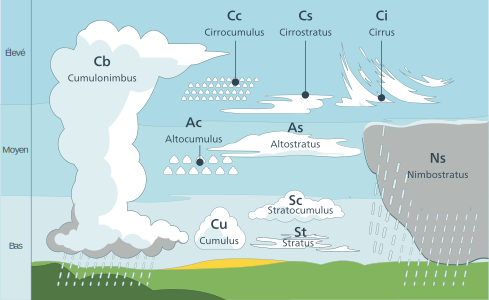
\includegraphics[width=0.75\textwidth]{03-Meteo/img/nuages.pdf}
    \legende{Répartition des types de nuages dans la troposphère}{img:nuages}
    \end{figure}	